
\begin{frame}{Chapter 4: RAG System Implementation}
    \begin{center}
        \Large{\textbf{Chapter 4}}\\
        \vspace{0.5em}
        \huge{\textbf{Retrieval-Augmented Generation}}\\
        \huge{\textbf{System Implementation}}\\
        \vspace{0.5em}
        \large{Bilingual Medical Knowledge Base Development}
    \end{center}
\end{frame}

\begin{frame}{4.1 Introduction to RAG}
    \textbf{Retrieval-Augmented Generation:}
    \begin{itemize}
        \item Combines stored knowledge with text generation capabilities
        \item Effective solution for LLM limitations:
        \begin{itemize}
            \item[-] Access to up-to-date information
            \item[-] Reduction of hallucinations
            \item[-] Domain-specific knowledge integration
        \end{itemize}
    \end{itemize}
    
    \vspace{1em}
    
    \textbf{Chapter Structure:}
    \begin{itemize}
        \item \textbf{Part 1:} English RAG system implementation
        \item \textbf{Part 2:} Bilingual system with Persian integration
    \end{itemize}
\end{frame}

% PART 1: English RAG System
\begin{frame}[plain]
    \begin{center}
        \Large{\textbf{Part 1}}\\
        \vspace{0.5em}
        \huge{\textbf{English RAG System}}\\
    \end{center}
\end{frame}

\begin{frame}{4.2 English Datasets}
    \begin{table}[h]
        \centering
        \footnotesize
        \caption{English Datasets for RAG System}
        \begin{tabular}{lccc}
            \toprule
            \textbf{Dataset} & \textbf{Domain} & \textbf{Count} & \textbf{Chunking} \\
            \midrule
            Wikipedia & General & 29.9M & Default \\
            PubMed & Biomedical & 23.9M & Default \\
            Textbooks & Medical & 125.8K & Default \\
            StatePearls & Clinical & 247K & Recursive + Late \\
            MedCorp & Various & 54.2M & Mixed \\
            \midrule
            \rowcolor{improvement!20} \textbf{Final Selection} & Medical & \textbf{373.5K} & - \\
            \bottomrule
        \end{tabular}
    \end{table}
    
    \begin{center}
        \textbf{Selected:} StatePearls + Textbooks (quality over quantity)
    \end{center}
\end{frame}

\begin{frame}{4.3 Late Chunking Technique}
    \textbf{Three-Phase Process:}
    
    \vspace{0.5em}
    
    \textbf{Phase 1: Recursive Chunking}
    \begin{itemize}
        \item Split by natural separators
        \item Size control with overlap
    \end{itemize}
    
    \textbf{Phase 2: Simultaneous Vector Generation}
    \begin{itemize}
        \item Process all chunks together
        \item Preserve inter-chunk relationships
    \end{itemize}
    
    \textbf{Phase 3: Aggregation and Pooling}
    \begin{itemize}
        \item Process entire document first
        \item Generate unified representation
        \item Split vector by boundaries
    \end{itemize}
    
    \begin{center}
        \colorbox{highlight!20}{\textbf{Key: Full context preserved in each chunk}}
    \end{center}
\end{frame}

\begin{frame}{Late Chunking Architecture}
    \begin{center}
        % Placeholder for the actual image
        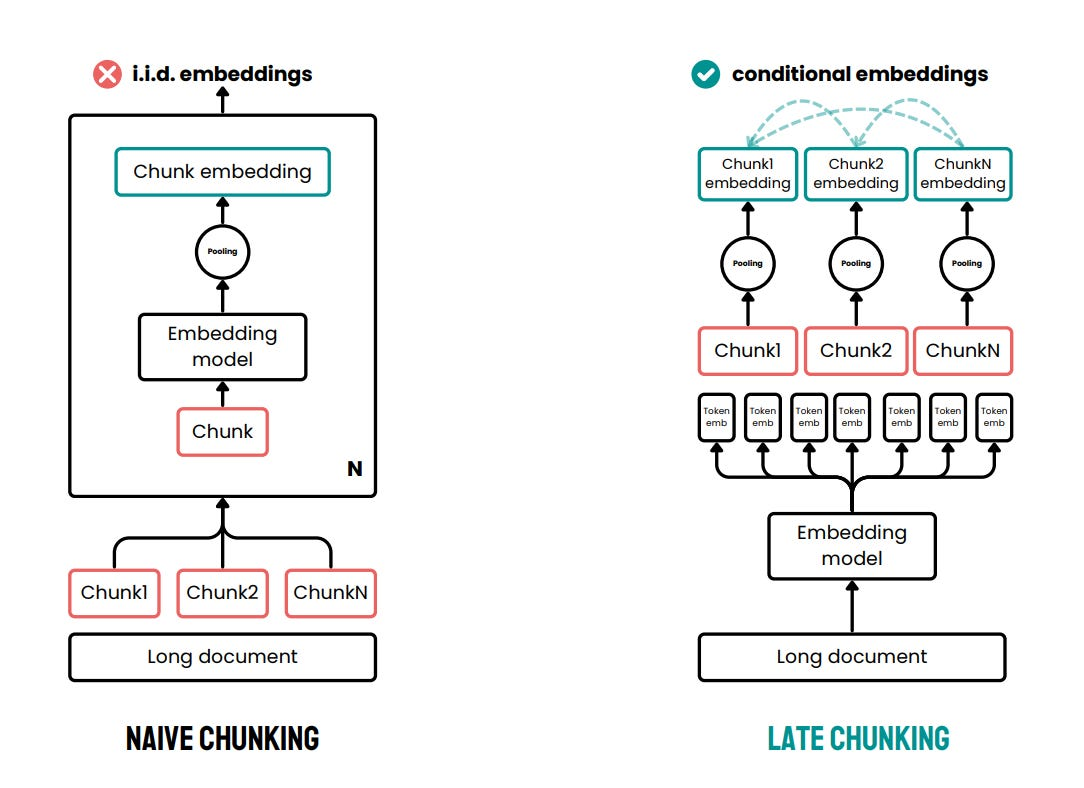
\includegraphics[width=0.9\textwidth]{images/late-chunking}
        % If image not available, use placeholder:
        % \fbox{
        %     \begin{minipage}{0.9\textwidth}
        %         \centering
        %         \vspace{3cm}
        %         \textit{[Late Chunking Architecture Diagram]}\\
        %         \vspace{3cm}
        %     \end{minipage}
        % }
        
        \vspace{0.5em}
        \textbf{Traditional:} Chunk → Embed → Store\\
        \textbf{Late Chunking:} Full Document → Embed → Chunk → Store\\
        
        \vspace{0.5em}
        \colorbox{improvement!20}{15-20\% improvement in retrieval accuracy}
    \end{center}
\end{frame}

\begin{frame}{4.4 English System Configuration}
    \begin{columns}[T]
        \column{0.5\textwidth}
        \textbf{Chunking Parameters:}
        \begin{itemize}
            \item StatePearls: 1024 chunk size
            \item Overlap: 100 tokens
            \item Method: Recursive + Late
            \item Textbooks: 300 chunk size
        \end{itemize}
        
        \column{0.5\textwidth}
        \textbf{Storage Architecture:}
        \begin{itemize}
            \item Elasticsearch backend
            \item Full-text search
            \item Vector search
            \item Hybrid search capability
        \end{itemize}
    \end{columns}
\end{frame}

\begin{frame}{4.5 English RAG Results}
    \begin{table}[h]
        \centering
        \tiny
        \caption{English Model Performance with/without RAG}
        \begin{tabular}{l|cccccccc}
            \toprule
            \textbf{Model} & \textbf{HeadQA} & \textbf{MedQA} & \textbf{MedMCQA} & \textbf{Anat.} & \textbf{C-K} & \textbf{C-M} & \textbf{MG} & \textbf{PM} \\
            \midrule
            gemma-3-12b-it & 70.97 & 65.06 & 55.23 & 65.19 & 75.10 & 75.35 & 78.79 & 78.66 \\
            gemma-3-12b-it-en-sft & 77.33 & 74.28 & 61.46 & 70.38 & 80.72 & 80.83 & 82.82 & 81.65 \\
            \rowcolor{improvement!20} + RAG & 78.83 & 75.42 & 62.20 & 71.56 & 82.10 & 83.12 & 82.50 & 82.46 \\
            \bottomrule
        \end{tabular}
    \end{table}
    
    \vspace{0.5em}
    
    \begin{center}
        \textbf{Improvements:}\\
        +1.09\% vs fine-tuned model\\
        +6.73\% vs base model\\
        Highest gain in College Medicine (+2.29\%)
    \end{center}
\end{frame}

% PART 2: Bilingual RAG System
\begin{frame}[plain]
    \begin{center}
        \Large{\textbf{Part 2}}\\
        \vspace{0.5em}
        \huge{\textbf{Bilingual RAG System}}\\
    \end{center}
\end{frame}

\begin{frame}{4.6 Persian Integration}
    \textbf{Motivation:}
    \begin{itemize}
        \item Lack of credible Persian medical resources
        \item Need to serve Persian-speaking users
    \end{itemize}
    
    \vspace{0.5em}
    
    \textbf{Persian Medical Corpus:}
    \begin{itemize}
        \item Comprehensive Persian medical content
        \item Collected from credible domestic sources
        \item Processed with Hazm library
    \end{itemize}
\end{frame}

\begin{frame}{4.7 Bilingual Dataset Overview}
    \begin{table}[h]
        \centering
        \footnotesize
        \caption{Complete Bilingual RAG System Datasets}
        \begin{tabular}{lcccc}
            \toprule
            \textbf{Dataset} & \textbf{Language} & \textbf{Original} & \textbf{Chunks} & \textbf{Method} \\
            \midrule
            Textbooks & English & 125.8K & 125.8K & Default \\
            StatePearls & English & 247K & 247K & Recursive + Late \\
            \rowcolor{highlight!20} Persian Medical & Persian & 102K & 5,176,679 & Recursive + Late \\
            \midrule
            \textbf{Total} & Bilingual & - & \textbf{5,550,179} & - \\
            \bottomrule
        \end{tabular}
    \end{table}
    
    \begin{center}
        \colorbox{improvement!20}{\textbf{Over 5.5 million chunks in bilingual system}}
    \end{center}
\end{frame}

\begin{frame}{4.8 Persian Processing}
    \textbf{Preprocessing with Hazm:}
    \begin{itemize}
        \item Text normalization
        \item Sentence boundary detection
        \item Appropriate tokenization
    \end{itemize}
    
    \vspace{0.5em}
    
    \textbf{Chunking Configuration:}
    \begin{itemize}
        \item Method: Recursive + Late Chunking
        \item Generated 5,176,679 chunks
        \item Max chunk: 500 characters
        \item Overlap: 100 characters
    \end{itemize}
\end{frame}

\begin{frame}{4.9 Bilingual Challenges}
    \textbf{Cross-lingual Retrieval Challenge:}
    
    \begin{itemize}
        \item Users ask in Persian, documents in English (and vice versa)
        \item Traditional methods (TF-IDF, BM25) fail in bilingual context
    \end{itemize}
    
    \vspace{0.5em}
    
    \textbf{Solution:}
    \begin{center}
        \colorbox{highlight!20}{\textbf{Cosine similarity on multilingual embeddings}}
    \end{center}
    
    \vspace{0.5em}
    
    \textbf{Benefits:}
    \begin{itemize}
        \item Cross-lingual semantic understanding
        \item Unified knowledge base management
        \item Implicit concept translation
    \end{itemize}
\end{frame}

\begin{frame}{4.10 Persian RAG Results}
    \begin{table}[h]
        \centering
        \footnotesize
        \caption{Persian Model Performance with/without RAG}
        \begin{tabular}{l|ccccc}
            \toprule
            \textbf{Model} & \textbf{Anatomy} & \textbf{Clinical} & \textbf{College} & \textbf{Genetics} & \textbf{Prof.} \\
            \midrule
            gemma-3-12b-it (baseline) & 56\% & 68\% & 74\% & 72\% & 74\% \\
            gemma-3-12b-it-fa-sft & 58\% & 70\% & 76\% & 74\% & 76\% \\
            \rowcolor{improvement!20} + RAG & 60\% & 71\% & 77\% & 75\% & 77\% \\
            \bottomrule
        \end{tabular}
    \end{table}
    
    \vspace{0.5em}
    
    \begin{center}
        \textbf{Improvements:}\\
        +1.2\% vs fine-tuned model\\
        +3.2\% vs base model\\
        \vspace{0.5em}
        \textbf{Notable achievement with 5M+ Persian chunks}
    \end{center}
\end{frame}

\begin{frame}{4.11 System Performance Comparison}
    \begin{table}[h]
        \centering
        \caption{English vs Persian RAG Performance}
        \begin{tabular}{lcc}
            \toprule
            \textbf{Metric} & \textbf{English} & \textbf{Persian} \\
            \midrule
            Chunks & 373.5K & 5.17M \\
            Improvement vs Fine-tuned & +1.09\% & +1.2\% \\
            Improvement vs Base & +6.73\% & +3.2\% \\
            Best Domain Improvement & College Med (+2.29\%) & All domains (+1-2\%) \\
            \bottomrule
        \end{tabular}
    \end{table}
    
    \vspace{0.5em}
    
    \textbf{Key Achievement:}\\
    First comprehensive bilingual medical RAG system
\end{frame}

\begin{frame}{4.12 Technical Limitations}
    \textbf{Computational Constraints:}
    \begin{itemize}
        \item Response latency from 5.5M chunks
        \item Storage requirements (~15GB)
        \item Architecture complexity for bilingual management
    \end{itemize}
    
    \vspace{0.5em}
    
    \textbf{Design Decisions:}
    \begin{itemize}
        \item Excluded Wikipedia (29.9M) and PubMed (23.9M) due to size
        \item Focus on quality over quantity
        \item Optimized for medical domain specificity
    \end{itemize}
\end{frame}

\begin{frame}{4.13 Future Improvements}
    \begin{columns}[T]
        \column{0.5\textwidth}
        \textbf{Technical:}
        \begin{itemize}
            \item Graph RAG implementation
            \item Specialized medical embeddings
            \item Smart indexing optimization
        \end{itemize}
        
        \column{0.5\textwidth}
        \textbf{Knowledge Base:}
        \begin{itemize}
            \item More Persian medical sources
            \item Auto-translation of quality content
            \item Continuous updates
            \item Domain gap filling
        \end{itemize}
    \end{columns}
    
    \vspace{1em}
    
    \begin{center}
        \colorbox{highlight!20}{\textbf{Effective bilingual medical AI assistant achieved}}
    \end{center}
\end{frame}
